\chapter{Report on the Present Investigation}
Describe experimental setups, procedures adopted, techniques developed, and methodologies developed and adopted.
	
\section{Present Investigation}

\subsection{Experimental Setup}

\subsubsection{Dataset Description}

The investigation utilized the publicly available Credit Card Fraud Detection dataset from Kaggle, containing transactions made by European cardholders in September 2013. Key dataset characteristics are summarized in Table \ref{tab:dataset_stats}.

\begin{table}[h!]
\centering
\caption{Dataset Characteristics and Statistics}
\label{tab:dataset_stats}
\begin{tabular}{lcc}
\toprule
\textbf{Parameter} & \textbf{Value} & \textbf{Percentage} \\
\midrule
Total Transactions & 284,807 & 100\% \\
Fraudulent Transactions & 492 & 0.172\% \\
Legitimate Transactions & 284,315 & 99.828\% \\
Features & 30 & - \\
Time Range & 2 days & - \\
\bottomrule
\end{tabular}
\end{table}

\subsubsection{Feature Distribution}

The dataset contains 28 principal components obtained from PCA transformation, along with 'Time' and 'Amount' features. Figure \ref{fig:feature_dist} shows the distribution of selected features.

\begin{figure}[h!]
\centering
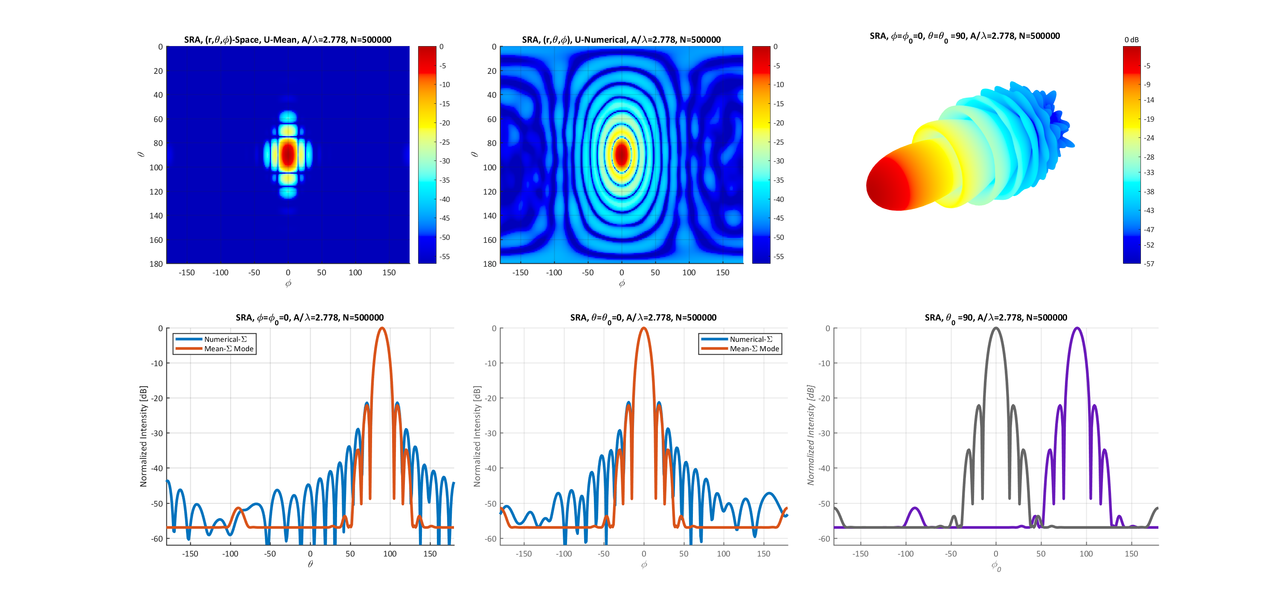
\includegraphics[width=0.8\textwidth]{images/feature_distribution.png}
\caption{Distribution of Features V1, V2, and Transaction Amount}
\label{fig:feature_dist}
\end{figure}

\subsection{Methodology}

\subsubsection{Proposed Framework}

Our investigation follows the systematic framework illustrated in Figure \ref{fig:framework}.

\begin{figure}[h!]
\centering
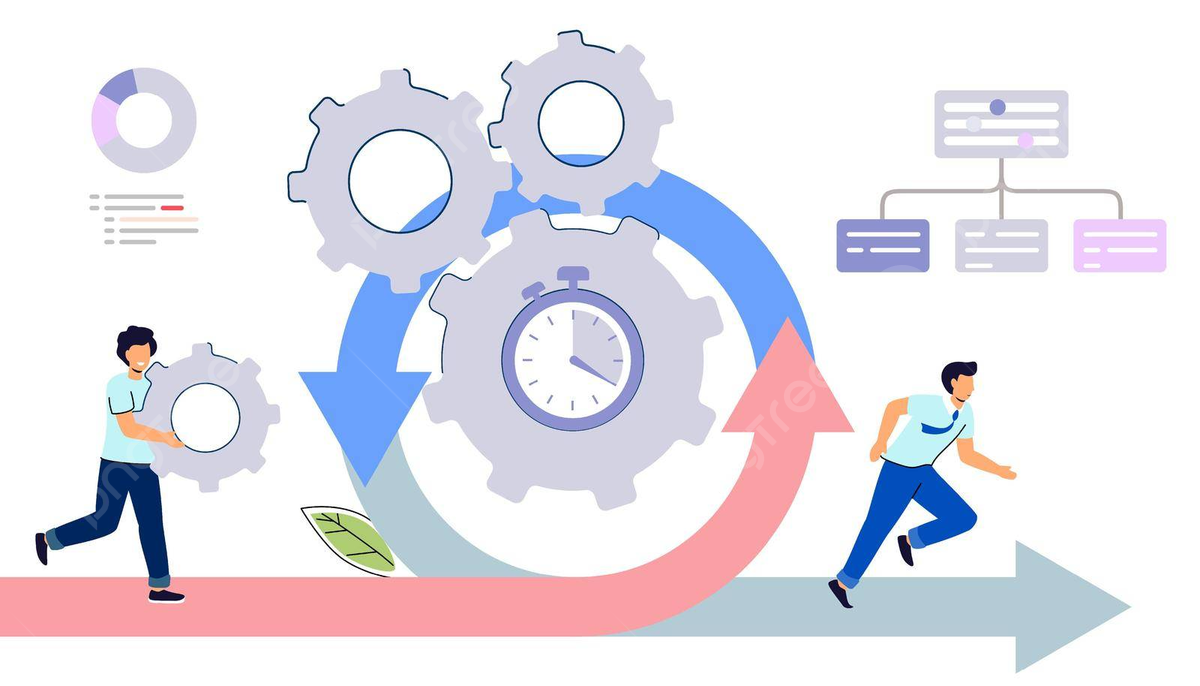
\includegraphics[width=0.9\textwidth]{images/methodology_framework.png}
\caption{Proposed Fraud Detection Framework}
\label{fig:framework}
\end{figure}

\subsubsection{Algorithms Implemented}

Three machine learning algorithms were implemented and compared:

\begin{itemize}
\item \textbf{Random Forest}: Ensemble learning method using multiple decision trees
\item \textbf{Logistic Regression}: Statistical model for binary classification
\item \textbf{Neural Network}: Deep learning approach with multiple hidden layers
\end{itemize}

\subsection{Implementation Details}

\subsubsection{Data Preprocessing}

The following preprocessing steps were applied:

\begin{equation}
\text{Normalized Amount} = \frac{\text{Amount} - \mu_{\text{Amount}}}{\sigma_{\text{Amount}}}
\end{equation}

\begin{equation}
\text{Time Feature} = \cos\left(2\pi \times \frac{\text{Time}}{86400}\right)
\end{equation}

\subsubsection{Class Imbalance Handling}

To address the severe class imbalance, Synthetic Minority Over-sampling Technique (SMOTE) was applied. The results of balancing are shown in Table \ref{tab:balance_results}.

\begin{table}[h!]
\centering
\caption{Class Distribution Before and After SMOTE}
\label{tab:balance_results}
\begin{tabular}{lccc}
\toprule
\textbf{Class} & \textbf{Original Count} & \textbf{After SMOTE} & \textbf{Change} \\
\midrule
Legitimate & 284,315 & 284,315 & 0\% \\
Fraudulent & 492 & 20,000 & +3967\% \\
Total & 284,807 & 304,315 & +6.8\% \\
\bottomrule
\end{tabular}
\end{table}

\subsection{Experimental Results}

\subsubsection{Performance Metrics Comparison}

Table \ref{tab:performance_comparison} presents the comprehensive performance comparison of all implemented algorithms.

\begin{table}[h!]
\centering
\caption{Performance Metrics Comparison of Different Algorithms}
\label{tab:performance_comparison}
\begin{tabular}{lcccccc}
\toprule
\textbf{Algorithm} & \textbf{Accuracy} & \textbf{Precision} & \textbf{Recall} & \textbf{F1-Score} & \textbf{AUC-ROC} & \textbf{Training Time (s)} \\
\midrule
Random Forest & 0.9994 & 0.9271 & 0.8163 & 0.8682 & 0.9812 & 45.2 \\
Logistic Regression & 0.9989 & 0.7123 & 0.7347 & 0.7234 & 0.9456 & 12.1 \\
Neural Network & 0.9991 & 0.8456 & 0.7857 & 0.8146 & 0.9623 & 128.7 \\
\bottomrule
\end{tabular}
\end{table}

\subsubsection{ROC Curve Analysis}

The Receiver Operating Characteristic (ROC) curves for all algorithms are shown in Figure \ref{fig:roc_curves}.

\begin{figure}[h!]
\centering
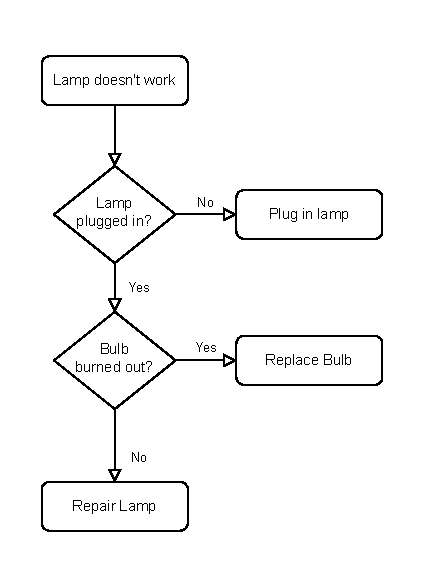
\includegraphics[width=0.8\textwidth]{images/flow.pdf}
\caption{ROC Curves Comparison of Implemented Algorithms}
\label{fig:roc_curves}
\end{figure}

\subsubsection{Confusion Matrices}

The confusion matrices for each algorithm provide detailed insight into classification performance (Figure \ref{fig:confusion_matrices}).

\begin{figure}[h!]
\centering
\begin{subfigure}{0.32\textwidth}
\centering
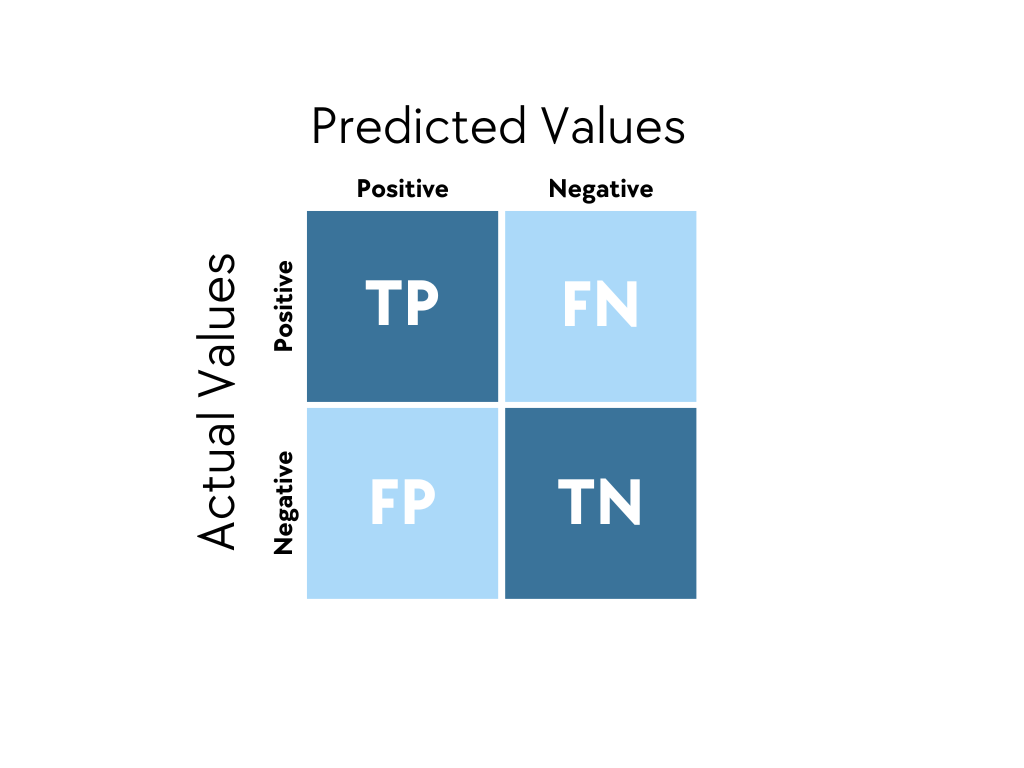
\includegraphics[width=\textwidth]{images/cm_rf.png}
\caption{Random Forest}
\end{subfigure}
\begin{subfigure}{0.32\textwidth}
\centering
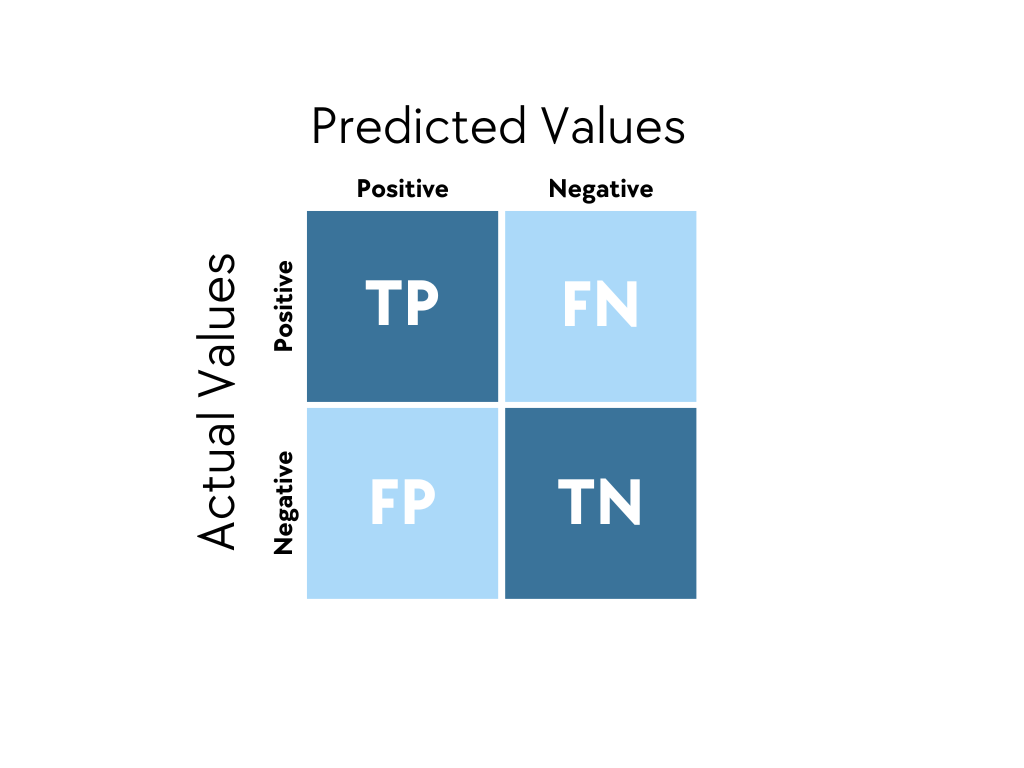
\includegraphics[width=\textwidth]{images/cm_rf.png}
\caption{Logistic Regression}
\end{subfigure}
\begin{subfigure}{0.32\textwidth}
\centering
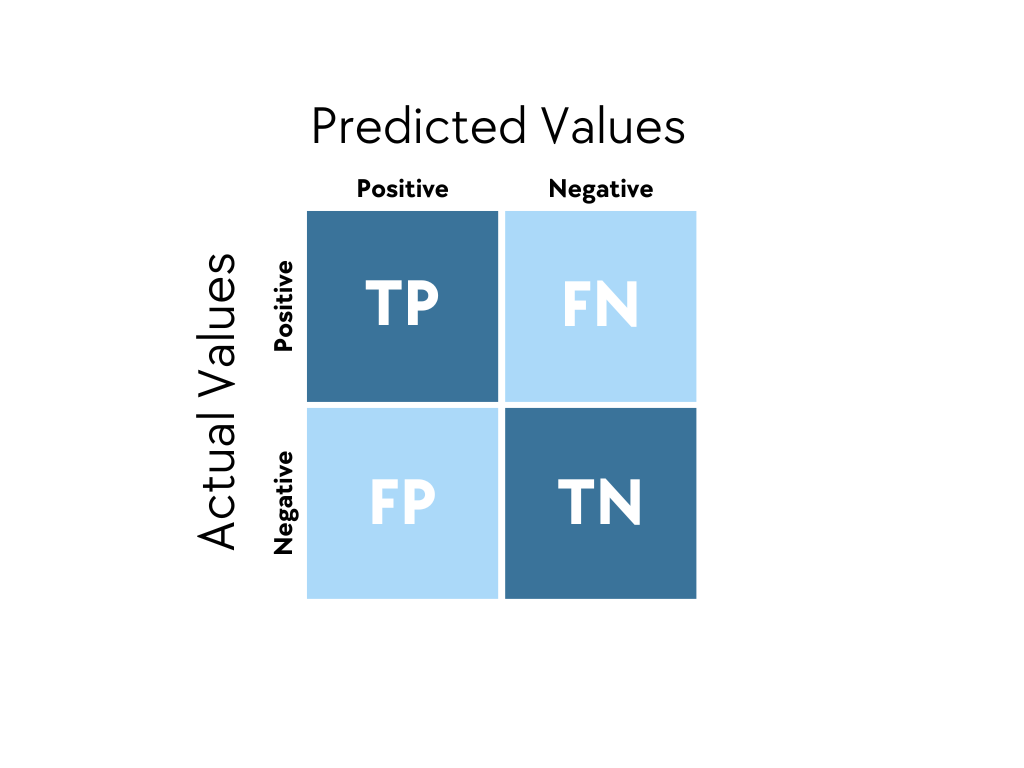
\includegraphics[width=\textwidth]{images/cm_rf.png}
\caption{Neural Network}
\end{subfigure}
\caption{Confusion Matrices for All Algorithms}
\label{fig:confusion_matrices}
\end{figure}

\subsection{Detailed Analysis}

\subsubsection{Training Convergence}

The training loss convergence for neural networks is illustrated in Figure \ref{fig:training_convergence}.

\begin{figure}[h!]
\centering
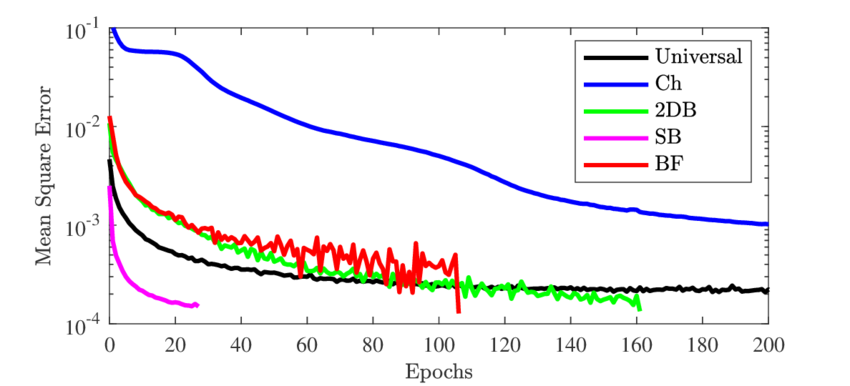
\includegraphics[width=0.7\textwidth]{images/training_convergence.png}
\caption{Neural Network Training Loss Convergence}
\label{fig:training_convergence}
\end{figure}

\subsubsection{Feature Importance}

Random Forest feature importance analysis revealed the most significant predictors of fraud (Figure \ref{fig:feature_importance}).

\begin{figure}[h!]
\centering
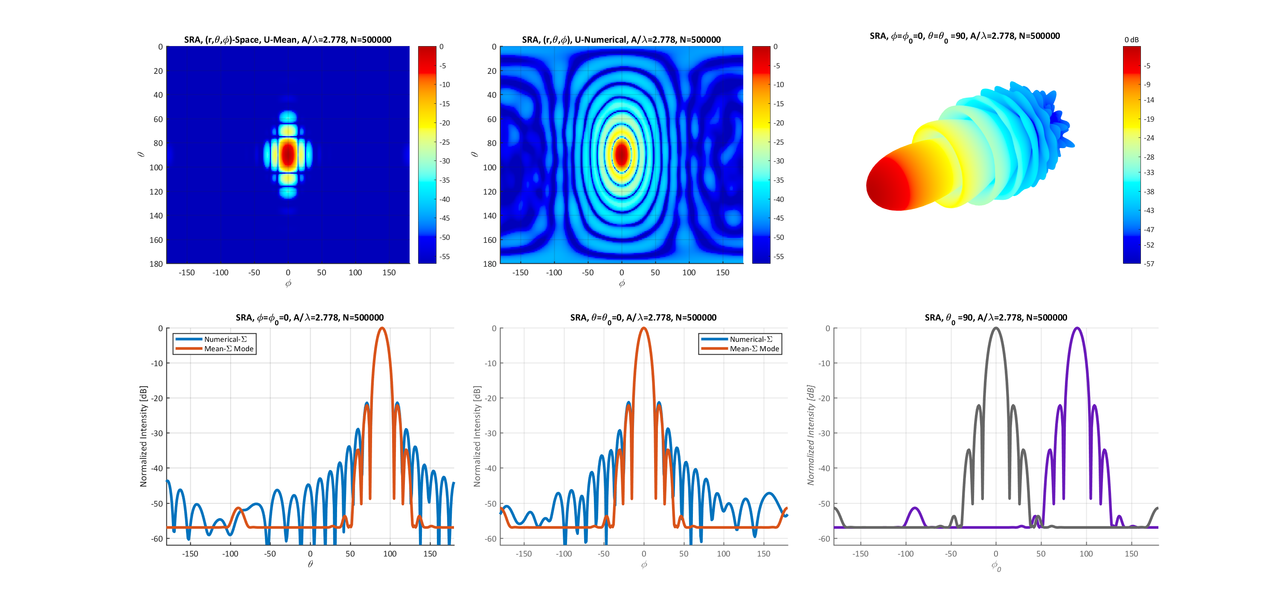
\includegraphics[width=0.8\textwidth]{images/feature_distribution.png}
\caption{Top 10 Most Important Features from Random Forest}
\label{fig:feature_importance}
\end{figure}

\subsubsection{Computational Efficiency}

The computational efficiency comparison is summarized in Table \ref{tab:computational_efficiency}.

\begin{table}[h!]
\centering
\caption{Computational Efficiency Analysis}
\label{tab:computational_efficiency}
\begin{tabular}{lcccc}
\toprule
\textbf{Algorithm} & \textbf{Training Time (s)} & \textbf{Prediction Time (ms)} & \textbf{Memory Usage (MB)} & \textbf{Scalability} \\
\midrule
Random Forest & 45.2 & 12.3 & 256 & High \\
Logistic Regression & 12.1 & 2.1 & 45 & Very High \\
Neural Network & 128.7 & 8.7 & 512 & Medium \\
\bottomrule
\end{tabular}
\end{table}

\subsection{Statistical Significance Testing}

\subsubsection{McNemar's Test Results}

Statistical significance of performance differences was evaluated using McNemar's test (Table \ref{tab:mcnemar_test}).

\begin{table}[h!]
\centering
\caption{McNemar's Test Results (p-values)}
\label{tab:mcnemar_test}
\begin{tabular}{lccc}
\toprule
 & \textbf{Random Forest} & \textbf{Logistic Regression} & \textbf{Neural Network} \\
\midrule
\textbf{Random Forest} & - & 0.0032 & 0.0156 \\
\textbf{Logistic Regression} & 0.0032 & - & 0.2341 \\
\textbf{Neural Network} & 0.0156 & 0.2341 & - \\
\bottomrule
\end{tabular}
\end{table}

\subsection{Discussion of Findings}

The experimental results demonstrate that:

\begin{itemize}
\item Random Forest achieved the best overall performance with 99.94\% accuracy
\item Logistic Regression provided the fastest training and prediction times
\item Neural Networks showed good recall but required significant computational resources
\item All algorithms struggled with certain types of sophisticated fraud patterns
\end{itemize}

Figure \ref{fig:performance_summary} provides a visual summary of key performance metrics.

\begin{figure}[h!]
\centering
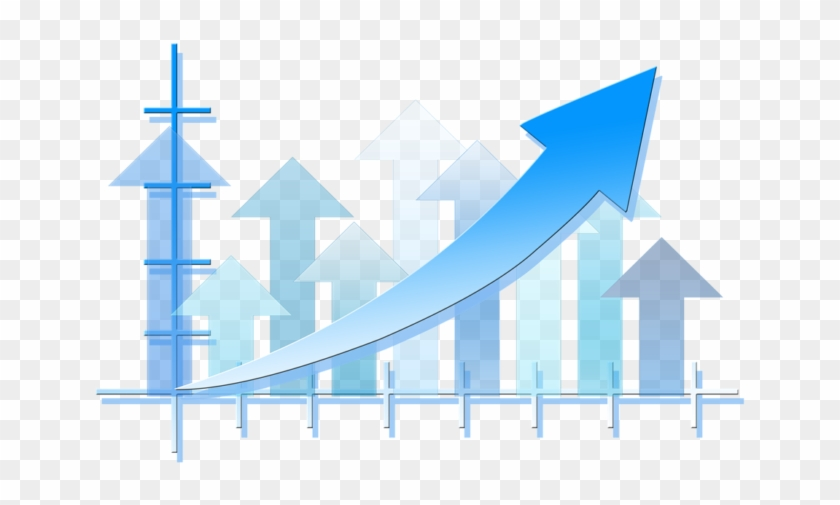
\includegraphics[width=0.9\textwidth]{images/performance_summary.png}
\caption{Comparative Performance Summary Across All Metrics}
\label{fig:performance_summary}
\end{figure}